\subsection{Design Constraints}

\subsubsection{Software Constraints}
\begin{enumerate}
	\item Device Accelerometer Support:
	\newline
	Given that a device does has an accelerometer, the device manufacturer must provide a software interface to interact with the device's accelerometer.
\end{enumerate}

\subsubsection{Hardware Constraints}
\begin{enumerate}
	\item Accelerometer:
	\newline
	Not all devices models are made equal. Some older devices do not have accelerometers to track steps with. The accuracy of accelerometers also vary from different device manufacturers.
	\item Battery Life:
	\newline
	To track steps continuously with a background process will greatly impact the battery life of devices with small battery capacities. 
\end{enumerate}

\subsection{Software System Attributes} 
\subsubsection{Reliability} 
The fitness module must be able to accurately and reliably track movement through the devices accelerometer. This accuracy and reliability ensures that the calculation of steps, calories and other health related data is accurate. The accuracy and reliability requirements are to ensure that milestones and awards are distributed accurately.    

\subsubsection{Efficiency} 
In order for the application to efficiently count steps and calculate other health metrics, the fitness module needs efficient algorithms to calculate the steps and other health metrics quickly from the data it recives from the accelerometer.  

\subsubsection{Portability} 
The fitness module should be able to work on both iOS and Android devices. There should also be no discernible differences between the fitness module on iOS and the fitness module on Android devices. They should also yield the same the same health metrics. 

\subsubsection{Coupling} 
The fitness module should also integrate with the user module. It should be able to request the users age and name. The fitness module should also be able to write data such as the users height and weight. Minimal helth metrics should also be sent to the user module to be stored on the server. 


\subsection{Activity Diagram}
See figure~\ref{fig:fitness_activity_diagram} on page~\pageref{fig:fitness_activity_diagram}
\begin{figure}
	\centering
	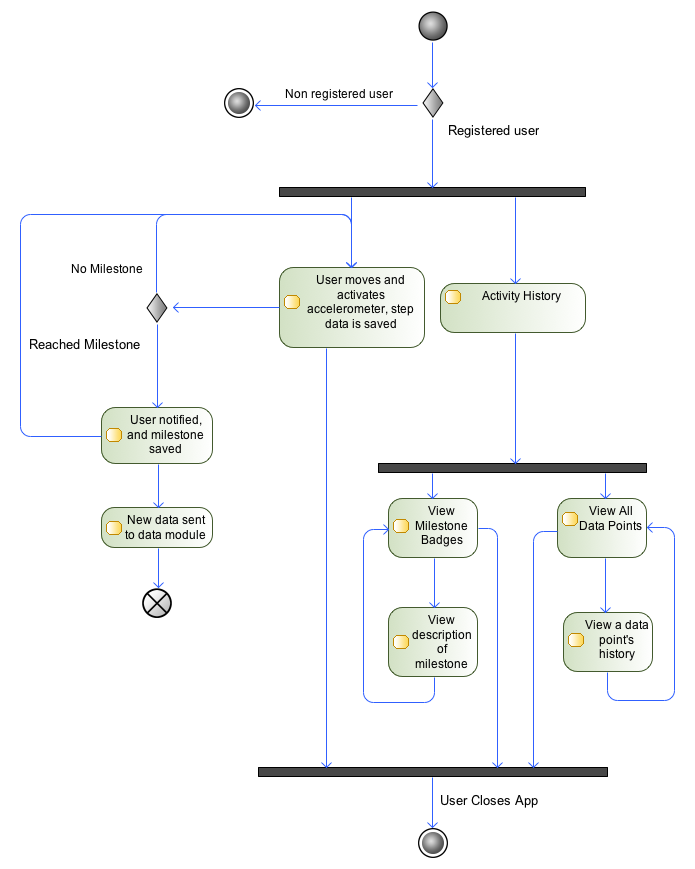
\includegraphics[scale=0.54]{Fitness/fitness_activity_diagram.png}
	\caption{Fitness Activity Diagram}
	\label{fig:fitness_activity_diagram}
\end{figure}

\subsection{State Diagrams}
See figure~\ref{fig:fitness_state_diagram} on page~\pageref{fig:fitness_state_diagram}
\begin{figure}
	\centering
	\includegraphics[scale=0.54]{Fitness/fitness_state_diagram.png}
	\caption{Fitness State Diagram}
	\label{fig:fitness_state_diagram}
\end{figure}

\subsection{Deployment Diagram}
See figure~\ref{fig:fitness_deployment_diagram} on page~\pageref{fig:fitness_deployment_diagram}
\begin{figure}
	\centering
	\includegraphics[scale=0.54]{Fitness/fitness_deployment_diagram.png}
	\caption{Fitness Deployment Diagram}
	\label{fig:fitness_deployment_diagram}
\end{figure}

\subsection{Class Diagram}
See figure~\ref{fig:Fitness_Class_Diagram} on page~\pageref{fig:Fitness_Class_Diagram}
\begin{figure}
	\centering
	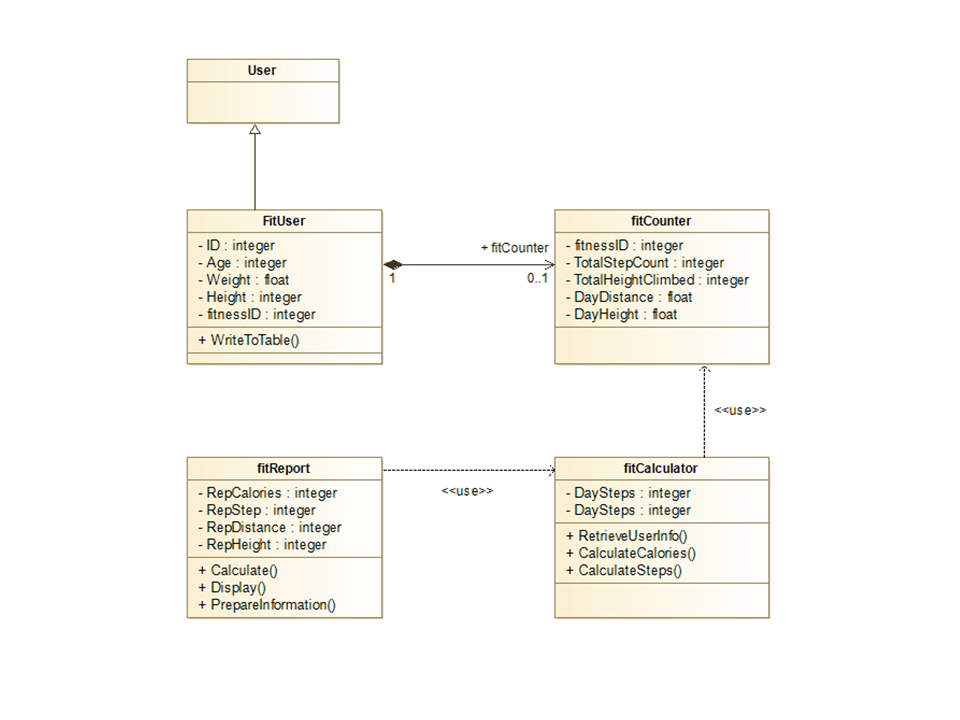
\includegraphics[scale=0.54]{Fitness/Fitness_Class_Diagram.png}
	\caption{Fitness Class Diagram}
	\label{fig:Fitness_Class_Diagram}
\end{figure}

\subsection{Sequence Diagram}
See figure~\ref{fig:Fitness_Sequence_Diagram} on page~\pageref{fig:Fitness_Sequence_Diagram}
\begin{figure}
	\centering
	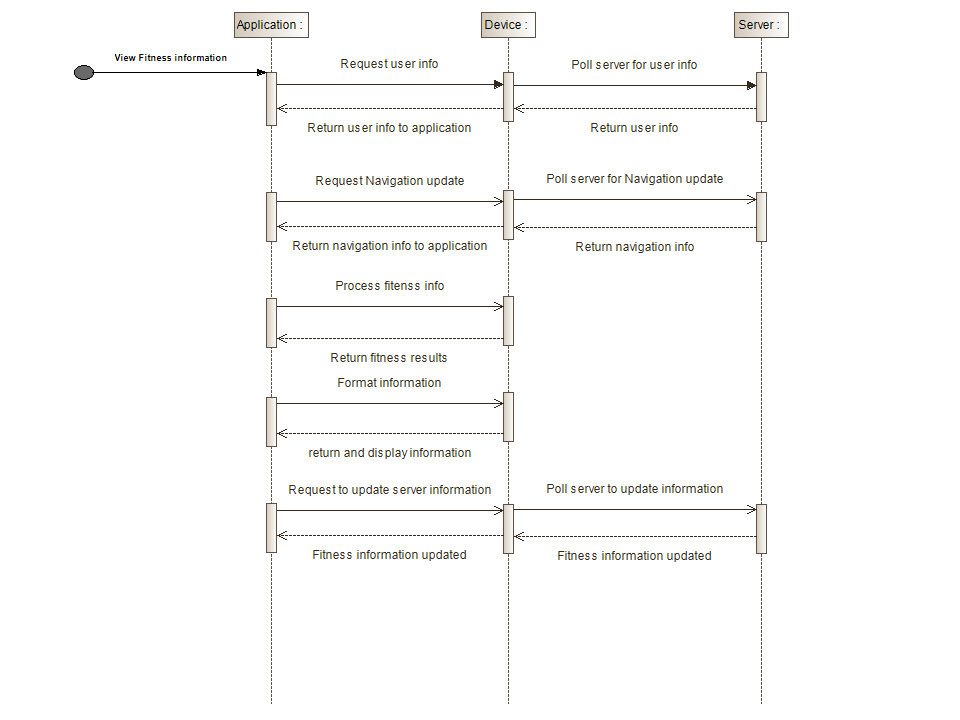
\includegraphics[scale=0.54]{Fitness/Fitness_Sequence_Diagram.png}
	\caption{Fitness Sequence Diagram}
	\label{fig:Fitness_Sequence_Diagram}
\end{figure}

\subsection{Use Case Diagram}
See figure~\ref{fig:Fitness_Use_Case_Diagram} on page~\pageref{fig:Fitness_Use_Case_Diagram}
\begin{figure}
	\centering
	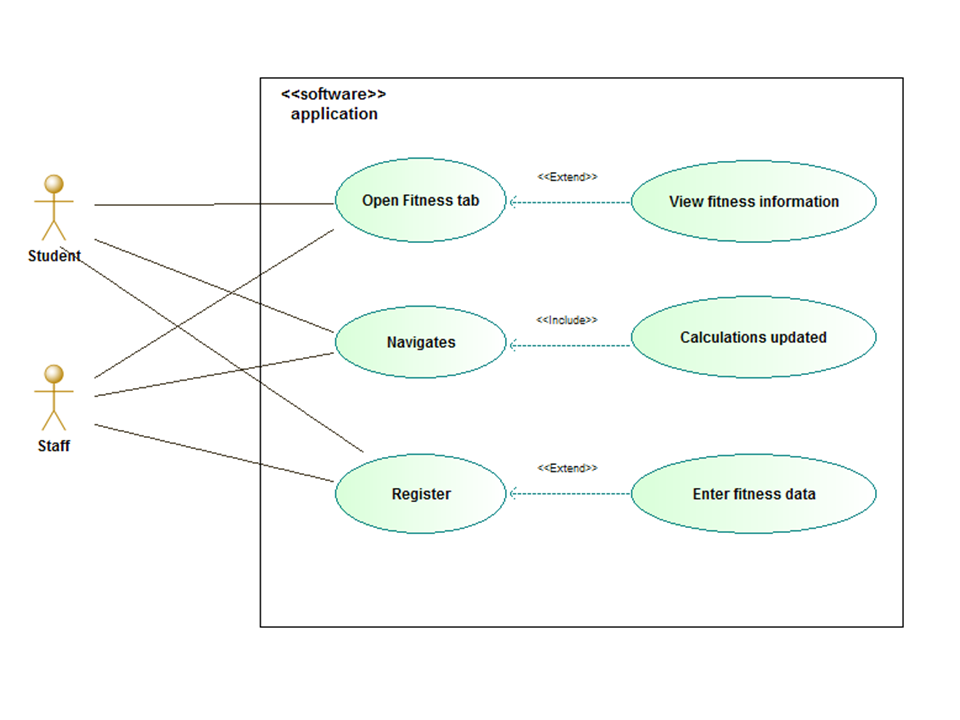
\includegraphics[scale=0.54]{Fitness/Fitness_Use_Case_Diagram.png}
	\caption{Fitness Use Case Diagram}
	\label{fig:Fitness_Use_Case_Diagram}
\end{figure}

\subsubsection{Performance Requirements}
\begin{enumerate}
	\item Tracking Information Accuracy
	\newline
	The tracking information that is obtained from the Navigation module needs to be as accurate as possible. This will ensure that the information calculated by the fitness module will be accurate and ensure that the user is presented with information that is not false.
	\item Server Storage
	\newline
	The information obtained from other modules and calculated inside the fitness module is to be stored on the server hosting the NavUP application. This means that the server will need to store certain fitness statistics and health information for roughly 60 000 users. The information will need to be able to be stored in a concurrent manner as to not create performance delays during application use.
	\newline
	By storing the fitness information on the server rather than keeping it on the handheld device, we avoid complications whereby the user might uninstall and reinstall the application. Situations whereby the user gets a new phone or performs any actions where there may be data loss can be dealt with in this manner because then information can be re-downloaded.  
	\newline
By storing fitness information on the server we can also provide a future integration where health-insurance companies could link to the database and use the information to provide some form of a reward system for the user based on his/her fitness achievements.  

\item The User Experience 
	\newline
All calculations with regards to fitness statistics and other fitness information is to be done on the device itself rather than using the application server. This will relieve the server of traffic and avoid a congested wireless network on campus. The user experience, with regards to local device calculations needs to be perceived as smooth and not be delayed by the calculations.

\item Communication transfer from phone to server
	\newline
Information transfer between the phone and the server is required to happen in a timely manner when the user requests to calculate fitness information. If the information were to take too long to be retrieved from the server to the phone then the user would have to wait longer than expected to see the fitness information.
	\newline
With these requirements of fast data transfers there becomes an inherent requirement with regards to the data being sent and retrieved. The data would have to be stored in a format of minimal size as to optimize the fore-mentioned process.


\item Reporting of fitness information
	\newline
The reporting part of the fitness module would need to be able to summarize, format and display certain information in a timely manner as to not delay the user interface thread. This would occur when the user selects the option to view his/her fitness information.

\end{enumerate}

\subsubsection{Performance Requirements}
\begin{enumerate}
	\item Tracking Information Accuracy
	\newline
	The tracking information that is obtained from the Navigation module needs to be as accurate as possible. This will ensure that the information calculated by the fitness module will be accurate and ensure that the user is presented with information that is not false.
\end{enumerate}



